\documentclass[twocolumn]{ctexart}
\usepackage{ctex}
\usepackage{amsmath}

%首行缩进两字符 利用\indent \noindent进行控制
\usepackage{indentfirst}
\setlength{\parindent}{2em}

%算法包
\usepackage{caption}
\usepackage{algorithm}
\usepackage{algorithmic}

%页边距包
\usepackage{geometry}
\geometry {left=2.0cm ,right=2.0cm,top=2.5cm,bottom=2.5cm}

%枚举
\usepackage{enumerate}

%算法input output
\renewcommand{\algorithmicrequire}{\textbf{Input:}} % Use Input in the format of Algorithm
\renewcommand{\algorithmicensure}{\textbf{Output:}} % Use Output in the format of Algorithm

%数学符号
\usepackage{amssymb}
\usepackage{wasysym}
%图片
\usepackage{graphicx}

%表格
\usepackage{booktabs}
\usepackage{multirow}

%Tikz画图
\usepackage{tikz}
\usetikzlibrary{arrows,graphs} %指明是图库
%\usegdlibrary
\begin {document}
	\title{Problem Set 4 Answer Sheet}
	\author{\textbf{151220131谢旻晖}}
	\date{}
	\maketitle
	
\section*{Problem 5.1}
\begin{algorithm}
	\caption{NON\_RECURSIVE\_DFS}
	\label{NON_RECURSIVE}
	\begin{algorithmic}[1]
		\STATE \textbf{procedure} DFSSweep(G)
		\STATE //初始化颜色为white
		\FOR{each vertex \textbf{v} in V}
			\STATE color[v]=white
		\ENDFOR
		\FOR{each vertex \textbf{v} in V}
		\IF{color[v]==white}
			\STATE dfs(v)
		\ENDIF
		\ENDFOR
		\STATE \textbf{end procedure}
		\STATE  
		\STATE  //子过程dfs
		\STATE \textbf{procedure} dfs(v)
			\STATE color[v] = gray
			\STATE stack.push(v)
			\WHILE {!stack.empty}
				\STATE	v=stack.top()
				\STATE v\_isfinished=true
				\FOR {each \textbf{u} in adj[v]}
					\IF{color[u]==white}
						\STATE color[u]=grey
						\STATE push(u)
						\STATE v\_isfinished=false
						\STATE \textbf{break}
					\ENDIF
					
					\IF{v\_isfinished}
						\STATE color[v]=black
						\STATE stack.pop() //把v出栈
					\ENDIF
				\ENDFOR
			\ENDWHILE
		\STATE \textbf{end procedure}		
	\end{algorithmic}
\end{algorithm}
\indent 算法见\textbf{Algorithm }\ref{NON_RECURSIVE}

\section*{Problem 5.2}
\indent 只可能是CE。
\indent 说明如下:在u发现之前v已经完成了遍历,也即点着色为u白色,v黑色,显然只可能是Cross Edge

\section*{Problem 5.3}
\indent 采用反证法证明,如果一个收缩图有从强连通片x到强连通片y的环,即有强连通片x到强连通片y的有向路径,同时也有强连通片y到强连通片x的有向路径,那么x与y就相互可达,这与x,y都是强连通片矛盾。


\section*{Problem 5.4}
\indent 第一次DFS不可以被替换为BFS,原因是:第一次DFS中每遍历完成一个点有一个post order的入栈操作,这是BFS不可完成的。\\

\indent 而第二次DFS仅仅是为了遍历而已,可以被替换为BFS。

\section*{Problem 5.5}
\noindent DFS树根v是割点的充要条件为:v有两棵及两棵以上子树。\\
\noindent 证明:\\
\indent $\Longrightarrow$:\\
\indent 采用反证法,如果结论不成立,那么v没有或有1棵子树。如果v没有子树,则图为平凡图或不连通图,显然v不是割点,矛盾;如果v只有一个子树,则去掉v之后剩下的图也显然连通,矛盾;所以v有两棵及两棵以上子树。\\
\indent $\Longleftarrow$: \\
\indent 显然成立,去掉v之后两棵子树不再连通了。

\section*{Problem 5.6}
\indent 仍然可以正确。$back(v)$的意义为v的所有子树的back edge能回溯到的最早的$discovertime$,当v可以回溯到更早的结点时,$back(v)$就被更新了,如果v不是割点,那么经过更新缩小后的$back(v)$一定不比$discovertime(v.parent)$大。所以$back(v)$初值往大里放缩,并没有影响。\\


\section*{Problem 5.7}
\noindent 1.\\
\indent 首先证明引理:若无向图G中各顶点的度均大于或等于2,则G中必有回路。证明:在图G中寻找一条最长路P, 并设其最后一个节点为v, 考察v的邻点.易知, v的所有邻点都在P上, 否则, 若u是v的一个不在P上的邻点, 则$P+v\leadsto u$是一条更长的路, 矛盾.由于G中每个顶点的度都大于等于2, 故v存在一个邻点x, 且x在P上, 但x与v在P上不相邻, 此时路$x\xrightarrow{P}v$与$v\leadsto x$的并就构成了一个环.\\
\indent 接着证明原命题:如果图中有度为1的点,那么删除任意一个这样的点之后G显然仍然连通;如果图中没有度为1的点,那么图中所有点的度数均$\ge2$,图必定存在环,删除环上的任意一点之后,G仍然连通。\\
\noindent2.\\
%\begin{tikzpicture}[>=stealth, every node/.style={circle, draw, minimum size=0.75cm}]
%\graph
%{
%	1 -> 2;
%	2 -> 3;
%	3 -> 1;
%};  
%\end{tikzpicture}
\begin{center}
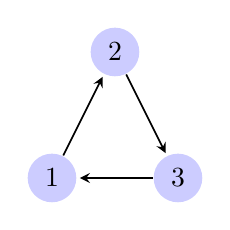
\begin{tikzpicture}
[> = stealth, % arrow head style
shorten > = 1pt, % don't touch arrow head to node
auto,
node distance = 3cm, % distance between nodes
semithick % line style
,scale=.8,auto=left,every node/.style={circle,fill=blue!20}]
\node (n1) at (0,0) {1};
\node (n2) at (1,2)  {2};
\node (n3) at (2,0)  {3};
\draw[->] (n1)->(n2);
\draw[->] (n2)->(n3);
\draw[->] (n3)->(n1);
\end{tikzpicture}
\end{center}

\noindent 3.\\
\begin{center}
	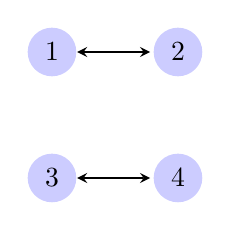
\begin{tikzpicture}[> = stealth, % arrow head style
	shorten > = 1pt, % don't touch arrow head to node
	auto,
	node distance = 3cm, % distance between nodes
	semithick % line style
	,scale=.8,auto=left,every node/.style={circle,fill=blue!20}]
	\node (n1) at (0,0) {1};
	\node (n2) at (2,0)  {2};
	\node (n3) at (0,-2)  {3};
	\node (n4) at (2,-2)  {4};
	\draw[<->] (n1)->(n2);
	\draw[<->] (n3)->(n4);
	\end{tikzpicture}
\end{center}




\section*{Problem 5.8}
\indent 当


\section*{Problem 5.10}
\indent 

\section*{Problem 5.11}


\section*{Problem 5.12}
\noindent 1.\\
\indent DFS(s),看是否可以遍历完所有点。\\

\noindent2.\\
\indent 使用SCC收缩有向图G,设收缩之后的DAG图为G'。对G'进行拓扑排序,对起点(排序为第一的)进行一次DFS,如果可以遍历完G'中的所有点,则存在这样一个"one-to-all"的顶点,否则不存在。\\
\indent 整体复杂度=SCC+拓扑排序+一次DFS=$O(m+n)$
\section*{Problem 5.13}
首先,可以很容易证明同一连通分量中的点的影响力值是相同的。\\
\noindent 1.\\
\indent STEP 1:对原图G,进行SCC收缩,形成分量收缩图G'。\\
\indent STEP 2:找到出度为0的那些连通分量收缩点,其中包含最少点数的那个连通分量中所有的点是影响力最小的点。\\
\indent 整体复杂度$=O(m+n)+O(n)+O(n)=O(m+n)$。\\
\noindent 2.\\
\indent STEP 1:对原图G,进行SCC收缩,形成分量收缩图G'。\\
\indent STEP 2:找到入度为0的那些连通分量收缩点,对其中的每个收缩点的某一点$x$进行一次DFS,同时记录下这个$x$可达的顶点个数,(其实也是该$x$所属的连通分量中任意一点的影响力)。\\
\indent STEP 3:找出其中影响力最大的连通分量,该分量中任意一点都是影响力最大的点。\\

\section*{Problem 5.16}
\noindent 1.\\
\indent 将问题建成图模型,每个小孩子都是一个顶点,如果"i恨j",则向图中添加一条$i\rightarrow j$的有向边,最终形成的图为G。\\
\indent
对G进行逆拓扑排序,若可以成功完成排序,则逆拓扑序就是小孩排队的顺序,否则,G存在环,不存在符合条件的排队方法。\\

\noindent 2.\\
\indent 将问题建成图模型,每个小孩子都是一个顶点,如果"i恨j",则向图中添加一条$i\rightarrow j$的有向边,最终形成的图为G。\\
\indent
求出G的关键路径长度,
\section*{Problem 5.17}
 


\section*{Problem 5.19}
\noindent (1)\\
\indent 可以的,我们设图的两部分可以最终被着色为蓝和红色。我们从任意一点开始,把他染成蓝色,进行无向图的DFS。\\
\indent 在DFS的过程中:$preorder$部分,将该结点染成\textbf{非}父结点颜色的颜色;每当即将访问一个已经访问过的点(Check NonTree Edge),检测该点与自身是否颜色不同,如果相同,则该图不是二部图。完成遍历之后,判定该图为二部图。\\
\noindent (2)\\
\indent \textbf{从处理角度来看:}DFS在有$post order$后序的处理时有优势,BFS则没有后序处理。\\
\indent \textbf{从问题类型来看:}DFS对于解决遍历和求所有问题有效,对于问题搜索深度小的时候处理速度迅速,然而在深度很大的情况下效率不高;BFS对于解决最短或最少问题特别有效,而且寻找深度小。\\
\section*{Problem 5.22}

\section*{Problem 5.24}

\section*{Problem 5.25}

\end {document}